\section{Route Validity Faults}\label{sec:validity}

BGP should satisfy {\em route validity}, as defined formally in
Chapter~\ref{chap:rlogic} (Definition~\ref{defn:rv}).
%BGP configuration affects which routes each router accepts, selects, and
%readvertises.  
Table~\ref{tab:rcc_tests} summarizes the route validity faults that \rcc
checks.  The biggest challenge for checking route validity is
that the definition says that the routes the routers in an AS select
should induce only policy-conformant paths (see
Definition~\ref{defn:pcp}), but \rcc operates without a specification of
the intended policy.  This section focuses on \rccns's approach to
detecting potential policy-related problems.

Requiring operators to provide a high-level policy specification would
require designing a specification language and convincing operators to
use it, and it provides no guarantees that the results would be more
accurate, since errors may be introduced into the specification itself.
Instead, \rcc forms {\em beliefs} about a network operator's intended
policy in two ways: (1)~assuming that intended policies conform to best
common practice and (2)~analyzing the configuration for common patterns
and looking for deviations from those patterns.  (The idea of forming
beliefs about intended protocol behavior is inspired from similar ideas
in systems~\cite{Engler01}.)  \rcc then finds cases
where the configuration appears to violate these beliefs.  It is
noteworthy that, even in the absence of a policy specification, this
technique detects many meaningful configuration faults and generates few
false positives.

%% An AS's customers will sometimes advertise smaller prefixes to its upstream
%% AS to load balance its inbound traffic, but it will tag those prefixes
%% with an instruction to its upstream to not readvertise these
%% prefixes~\cite{rfc1997}.  The export policies on an AS's routers should
%% always ensure that such a route is not readvertised to any neighbors.
%% Network operators also control the export of routes between
%% their peers and providers.  Static analysis can check this property by
%% analyzing the configuration files to verify that every eBGP session has
%% a filter that matches routes that have this instruction and prevents
%% them from being readvertised to other ASes.

\subsection{Violations of Best Common Practice}

We can derive some notions of high-level policy from our knowledge of
best common practice (\ie, the manner in which many ASes
tend to configure their 
networks).  In particular, \rcc looks for two violations of best common
practice: (1)~advertising a route from one ``peer'' to another (\ie, a
violation of the common business practices defined in
Table~\ref{tab:business} (Section~\ref{sec:semantics}); and (2)~not
advertising routes in a consistent manner at all peering
points~\cite{Feamster2004b}.  In this section, we explain both of these
practices in more detail.

A route that an AS learns from one of its ``peers'' should not be
readvertised to another peer.  Checking this condition requires
determining how a route propagates through an AS.
Figure~\ref{fig:policy_closure} illustrates how \rcc performs this
check.  Suppose that \rcc is analyzing the configuration from AS $X$ and
needs to determine that no routes learned from AS $B$ are exported to
AS $A$.  First, \rcc determines all routes that AS $X$ exports to AS $A$,
typically a set of routes that satisfy certain constraints on their
attributes. For example, router $R_1$ may export to AS $A$ only routes
that are ``tagged'' with the label ``$1000$''.  As described in
Section~\ref{sec:conf}, ASes often assign such ``community'' labels to a
route to
control how other routers rank or filter it. \rcc then checks the {\em
import} policies for all sessions to AS $B$, ensuring that no import
policy will set route attributes on any incoming route that would place
it in the set of routes that would be exported to AS $A$.  To perform
this check, \rcc must know which of an AS's neighboring ASes are peers;
thus, this check requires this additional input from the network
operator.

Additionally, an AS should advertise routes with equally good attributes
to each peer at every peering point.  An AS should not advertise routes
with inconsistent attributes, since doing so may prevent its peer from
implementing ``hot potato'' routing:
If ASes $1$ and $2$ are
peers, then the export policies of the routers in AS $1$ should export
routes to AS $2$ that have equal AS path length and MED values.  If not,
router $X$ could be forced to send traffic to AS $1$ via router $Y$
(``cold potato'' routing).
This behavior typically violates peering
agreements.  Recent work has observed that this type of inconsistent
route advertisement sometimes occurs in practice~\cite{Feamster2004b}.

An AS's policies may violate this best common practice for two reasons.
First, an AS may apply different export policies at different routers to
the same peer.  Checking for consistent export involves comparing export
policies on each router that has an eBGP session with a particular peer.
Static configuration analysis is useful because it can efficiently
compare policies on 
many different routers.  In practice, this comparison is not
straightforward because differences in policy definitions are difficult
to detect by direct inspection of the distributed router configurations.
\rcc facilitates comparing export policies across sets of routers by
normalizing all of the export policies for an AS, as described in
Table~\ref{tab:if} (Section~\ref{sec:rcc_overview}).  Second, an iBGP
signaling partition can 
create inconsistent export policies because routes with equally good
attributes may not propagate to all peering routes.  For example,
consider Figure~\ref{f:ibgp_vis_violation} again.  If routers $W$ and
$Z$ both learn routes to some destination $d$, then route $W$ may learn
a ``better'' route to $d$, but routers $Y$ and $Z$ will continue to
select the less attractive route.  If routers $X$ and $Y$ readvertise
their routes to a peer, then the routes advertised by $X$ and $Y$ will
not be equally good.  Thus, \rcc also checks whether routers that
advertise routes to the same peer are in the same iBGP signaling
partition (as described in Section~\ref{sec:visibility}, \rcc checks for
all iBGP signaling partitions, but ones that cause inconsistent
advertisement are particularly serious).

\subsection{Configuration Anomalies}

\begin{figure}
\begin{center}
\begin{psfrags}
\psfrag{AS A}{AS $A$}
\psfrag{AS B}{AS $B$}
\psfrag{AS X}{{\LARGE AS $X$}}
\psfrag{R1}{$R_1$}
\resizebox{0.85\textwidth}{!}{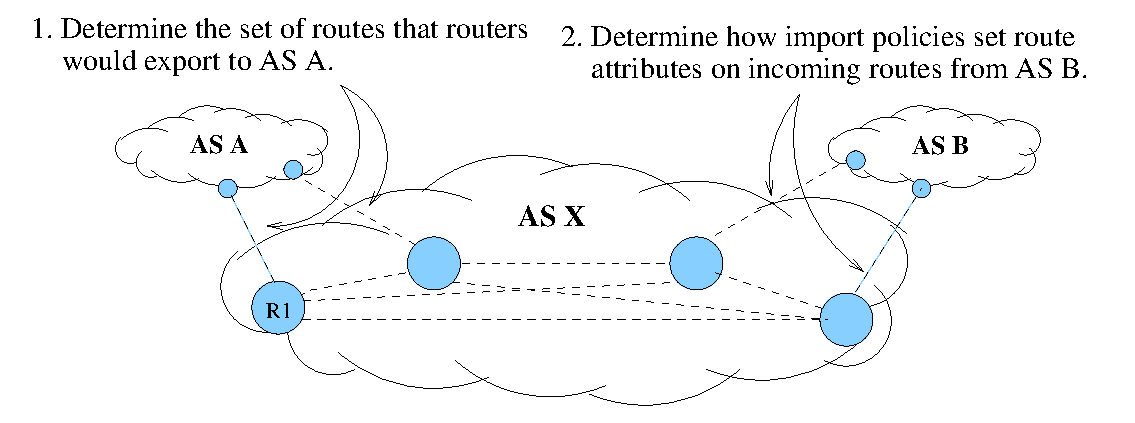
\includegraphics{rcc/figures/policy_closure.eps}}
\end{psfrags}
\end{center}
\caption{How \rcc computes route propagation.}
\label{fig:policy_closure}
\end{figure}

When the configurations for sessions at different routers to a
neighboring AS are the same except at one or two routers, the deviations
are likely to be mistakes.  This test relies on the belief that, if an
AS exchanges routes with a neighboring AS on many sessions and most of
those sessions have identical policies, then the sessions with slightly
different policies may be misconfigurations.  Of course, this test could
result in many false positives because there are legitimate reasons for
having slightly different import policies on sessions to the same
neighboring AS (\eg, outbound traffic engineering), but it does provide
a useful sanity check.

%% that all
%% routes received from a peer look equally good up to the IGP tiebreak
%% step, thus allowing it to use nearest exit (``hot potato'') routing with
%% its peers.  Of course, an AS cannot ensure that it receives AS paths of
%% equal length at all peering points with its peer, but it can take
%% precautions such as resetting the MED value on import and ensuring that
%% the local preference value is the same everywhere.  

